% Capítulo 2
\chapter{Capítulo 2}

\section{TTS}
\subsection{Breve história?}
\subsection{Approaches}
\subsubsection{Difones}
\subsubsection{HMM}
\subsubsection{Unit selection}
\subsubsection{DNN}
Falta de controle
\subsubsection{}
\section{Prosódia}
\subsection{Tipos de prosódia}
\subsubsection{Aumentativa}
\subsubsection{Outro tipo}
\subsubsection{Mais outro tipo}
\subsection{Prosódia como elemento extra-textual}
\subsection{Prosódia no português brasileiro}
\subsection{Trabalhos semelhantes?}

\section{Implementação}
\subsection{MBROLA}
\subsubsection{Formato}
\subsection{espeak-ng}
\subsection{Arquitetura}
Diagrama aqui
\subsection{Módulo de prosódia}
O programa foi codificado em Python em sua versão 3.6.Um editor gráfico de
prosódia foi programado utilizando as tecnologias web HTML, CSS, JavaScript.
\subsection{Linguagem prosódica}
A solução para melhorar a geração prosódica foi aumentar a linguagem, anotando
frases com marcadores de intenção.


\begin{figure}[!htbp]
\centering
\scalebox{0.65}{
    \begin{tikzpicture}[auto, >={Latex[inset=0pt, length=3mm, angle'=28,round]}, box/.style={draw,rounded corners,text width=3.0cm,align=center}]
    \node[] (txt) {Texto};
    \node[box, right=0.7cm of txt] (pre)
        {Pré-processador};
    \node[box, right=0.2cm of pre] (mor)
        {Analisador morfológico};
    \node[box, right=0.2cm of mor] (con)
        {Analisador de contexto};
    \node[box, right=of con] (let)
        {Módulo letra-som};
    \node[box, right=of let] (pro)
        {Gerador de prosódia};
        
    \draw[->] (txt) -- (pre);
        
    \node[box, fit=(pre)(mor)(con), label={[name=morfos_l] Analisador morfossintático}] (morfos) {};
    \node[box, fit=(let)] (letsom) {};
    \node[box, fit=(pro)] (proger) {};
    
    \node[inner sep=0, fit=(morfos)(letsom)(proger)] (all) {};
    \node[box,
          inner sep=0,
          yshift=-0.75cm,
          fit=(morfos.west)(proger.east),
          label=center:Estrutura de dados,
          minimum height=1cm,
          below of=all]
        (dad) {};
    
    \node[box, fit=(morfos)(morfos_l)(letsom)(proger)(dad), label=Processamento de linguagem natural] (nlp) {};
    
    \node[right=of dad, align=left] (out) {\emph{phones}\\ prosódia};
    
    \draw[->] (pre) -- (pre |- dad.north);
    \draw[<->] (mor) -- (mor |- dad.north);
    \draw[<->] (con) -- (con |- dad.north);
    \draw[<->] (let) -- (let |- dad.north);
    \draw[<->] (pro) -- (pro |- dad.north);
    
    \draw[->] (dad) -- (out);
        
    \end{tikzpicture}
}
\caption{Diagrama}
\label{fig:nlpdiagram}
\end{figure}

Este é o primeiro capítulo da parte central do trabalho, isto é, o desenvolvimento, a parte mais extensa de todo o trabalho. Geralmente o desenvolvimento é dividido em capítulos, cada um com subseções e subseções, cujo tamanho e número de divisões variam em função da natureza do conteúdo do trabalho.

Em geral, a parte de desenvolvimento é subdividida em quatro subpartes:
\begin{itemize}
	\item \textit{contextualização ou definição do problema} -- consiste em descrever a situação ou o contexto geral referente ao assunto em questão, devem constar informações atualizadas visando a proporcionar maior consistência ao trabalho;
	\item \textit{referencial ou embasamento teórico} -- texto no qual se deve apresentar os aspectos teóricos, isto é, os conceitos utilizados e a definição dos mesmos; nesta parte faz-se a revisão de literatura sobre o assunto, resumindo-se os resultados de estudos feitos por outros autores, cujas obras citadas e consultadas devem constar nas referências;
	\item \textit{metodologia do trabalho ou procedimentos metodológicos} -- deve constar o instrumental, os métodos e as técnicas aplicados para a elaboração do trabalho;
	\item \textit{resultados} -- devem ser apresentados, de forma objetiva, precisa e clara, tanto os resultados positivos quanto os negativos que foram obtidos com o desenvolvimento do trabalho, sendo feita uma discussão que consiste na avaliação circunstanciada, na qual se estabelecem relações, deduções e generalizações.
\end{itemize}

É recomendável que o número total de páginas referente à parte de desenvolvimento não ultrapasse 60 (sessenta) páginas.

\section{Seção 1}

Teste de figura:

\begin{figure}[htb]
	\centering
  	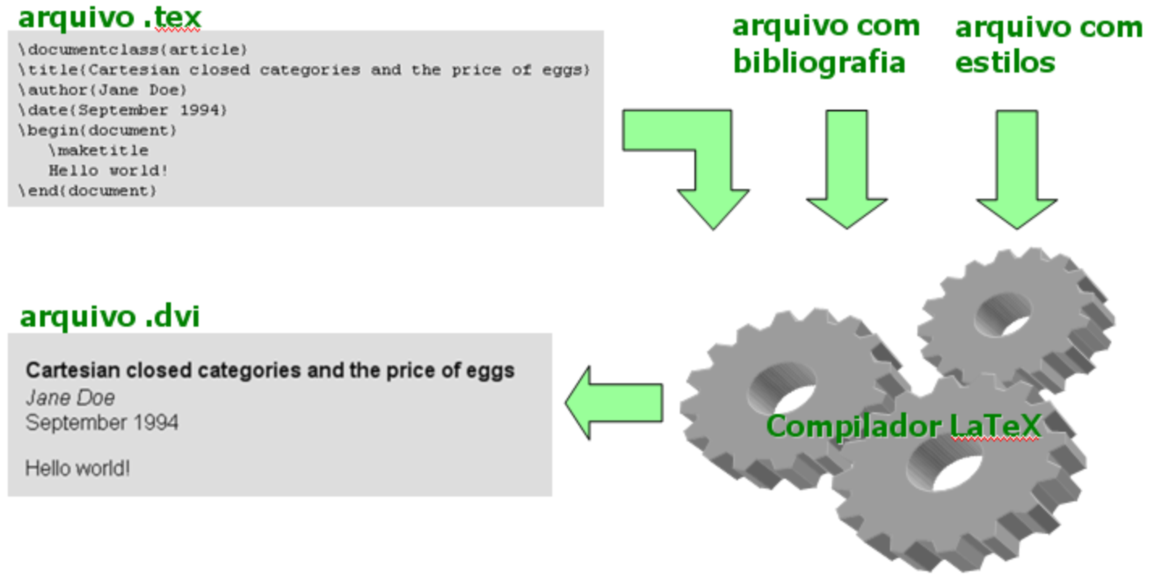
\includegraphics[scale=7.0]{Imagens/FiguraTeste.png}
  	\textsf{\caption{Teste de uma figura em formato .png}}
  	\label{fig:FiguraTeste}
\end{figure}


\section{Seção 2}

Referenciamento da figura inserida na seção anterior: \ref{fig:FiguraTeste}


\section{Seção 3}

Seção 3


\section{Seção 4}

Seção 4
